\documentclass[10pt,a4paper,notitlepage,oneside,twocolumn]{abst_jsarticle}
% notitlepage : \titlepage は独立しない
% oneside : 奇数・偶数ページは同じデザイン
% twocolumn : 2段組
% \setlength{\textwidth}{\fullwidth}
% 本文領域はページ一杯で, 傍注の幅を取らない

\usepackage[dvipdfmx]{graphicx, color}
% \usepackage{amsmath}
\usepackage{amsmath,amssymb}
\usepackage{comment}

\usepackage{url}
\usepackage{bm}
\usepackage{here}
\usepackage{algorithm}
\usepackage{algpseudocode}
\usepackage{hhline} 
\usepackage[hang,small,bf]{caption}
\usepackage[subrefformat=parens]{subcaption}
% \usepackage{tabularx}
% \usepackage[dvipdfm]{graphicx}
%\numberwithin{equation}{section}

\usepackage[hmargin=2truecm, textheight= 78zw]{geometry}
\columnsep=\dimexpr \textwidth - 50zw \relax

%%\unitlength=1pt
%%\renewcommand{\baselinestretch}{0.8}

\title{
{\bf 超高解像度の煙シミュレーションの高速化}
}

\author{\begin{center}
{\large {\bf 23N8100018BC 須之内 俊樹}}\\
{\large {\bf 情報工学専攻 形状情報処理研究室}}\\
{\large {\bf 2023年7月}}
\end{center}}

\date{}
\pagestyle{empty}

\begin{document}

\maketitle
%%%%%%%%%%%%%%%%%%%%%%%%%%%%%%
%\begin{figure*}[h]
%\begin{minipage}[t]{0.5\linewidth}
% \centering
%  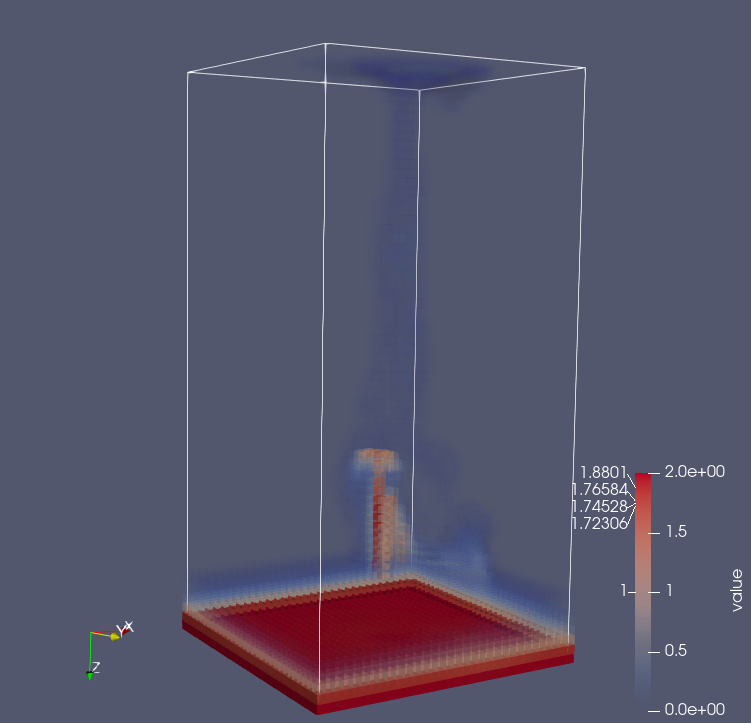
\includegraphics[height=5cm,width=5cm]{fd_conf_73.png}
%  \subcaption{前進差分を用いて計算した密度分布}
%  \label{fig:fig1}
%  \end{minipage}
%  \begin{minipage}[t]{0.5\linewidth}
%  \centering
%  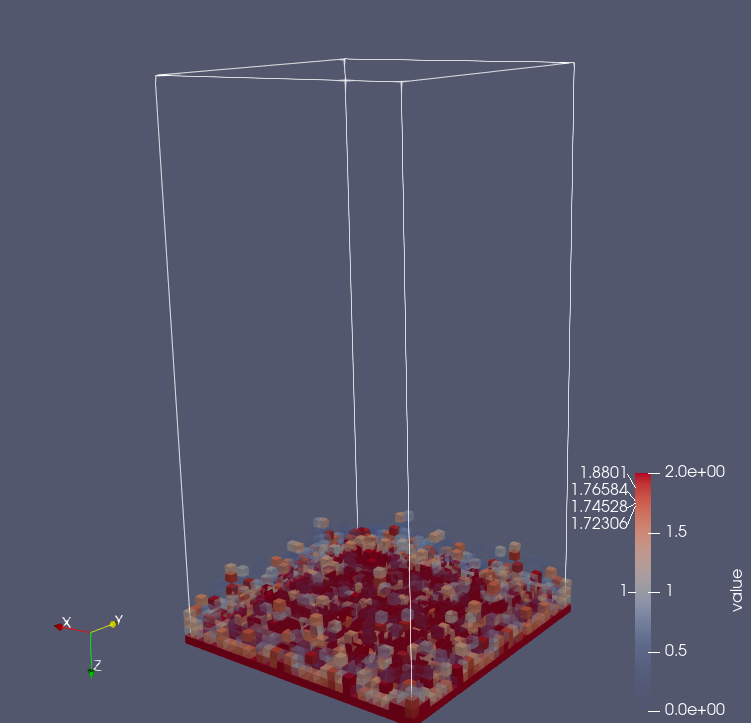
\includegraphics[height=5cm,width=5cm]{cd_smoke.png}
%  \subcaption{中心差分を用いて計算した密度分布}
%  \label{fig:fig2}
%  \end{minipage}
%\end{tabular}
%\caption{シミュレーションの密度分布を,ボクセルごとに密度によって色と透明度を色付けした.色が赤いほど密度が高く,青いほど密度が小さい.密度に従って透明度も変化させている.}
%\label{fig}
%\end{figure*}
\section{流体シミュレーション} \label{sec:intro}
流体の運動を記述する数理モデルの近似解を求めることを,流体シミュレーションという.計算機を使った流体力学を特別に,数値流体力学 (CFD: Computational Fluid Dynamics) と呼ぶ.CFDは実験で得ることが困難な流れ場全体の詳細な情報を得ることができる.CFDはCGによる流体の表現に役立っている.CGの分野では,流体の動きを忠実に再現することよりも,それらしい流体の運動を計算負荷を抑えて計算することが重視されている.流体の種類や運動によって条件を設けることで,よりそれらしい動きをシミュレーションすることができる.
次の2つの式を合わせてナビエ・ストークス方程式と呼び,これは流体力学の支配方程式である.非線形二階微分方程式となっており,代数的に一般解を求める事ができない.
\begin{equation}\label{eq:Navie}
\frac{\partial}{\partial t}\bm{u} = - (\bm{u} \boldsymbol{\cdot}\nabla) \bm{u} - \frac{1}{\rho}\nabla + \nu\nabla^2\bm{u} + \bm{f}
\end{equation}
%\begin{equation}\label{eq:uncompressed}
$$\nabla\boldsymbol{\cdot}\bm{u} = 0$$
%\end{equation}

数値流体力学ではシミュレーションする空間や時間を離散化して近似解を求める.空間の離散化は,各辺が空間の座標軸に並行な計算格子を用いて空間を分割し計算格子上に物理量を配置する格子法と,流体を粒子で表現し粒子上に物理量を配置する粒子法がある.ある時刻で空間の物理量の分布を計算した後,時刻を時間の刻み幅分進めて次の時刻の計算をすることを繰り返してシミュレーションを行う.

式\ref{eq:Navie}の右辺の第一項を移流項,第二項を圧力項,第三項を粘性項,第四項を外力項とよぶ.移流項は非線形項であり,その他は線形項である.
格子法における移流項の計算方法として,次の式で表されるStamのSemi-Lagrangian法\cite{semi-Lagrangian}がある.
%\begin{equation}\label{eq:semi-Lagrangian}
$$\bm{u}_{t+\Delta t}(\bm{x}_t) = \bm{u}_t(\bm{x}-\bm{u}_t(\bm{x}))$$
%\end{equation}
陽解法だと時間の刻み幅を大きくとると計算が安定しないが,Semi-Lagrangian法は陰解法であり,大きな時間の刻み幅に対応している.Semi-Lagrangian法は線形補間で容易に実装でき,CGでは広く用いられている.

圧力項の計算方法にChorinのprojection法\cite{projection}があり,仮の速度を$\bm{u}^*$として以下のポアソン方程式を解く.
\begin{equation}\label{eq:colin_p}
\nabla^2 \bm{p} =  \frac{1}{\Delta t}\nabla\boldsymbol{\cdot}\bm{u}^*
\end{equation} 
ノイマン境界条件は,$\frac{\partial p}{\partial \bm{n}} = 0$とする.これによりディリクレ境界条件も設定される.これはシミュレーション境界の格子に配置される,境界外の方向の速度成分を$0$とすることで実装できる.ポアソン方程式は離散化によって,線形方程式に帰着できる.シミュレーション領域の分割数を$n$とすると,行列は$n \times n$の疎行列になる.その後,次の式を用いて,次の時刻の速度を更新する.

%\begin{equation}\label{eq:colin_v}
$$\bm{u}_{t+\Delta t} = \bm{u}^* - \Delta t \nabla \bm{p}$$
%\end{equation} 

格子法では,流体を可視化する際は密度を元にレンダリングを行う.三次元空間において,モデルの表面のみのレンダリングをサーフェスレンダリングという.それに対し,モデルの透明度を計算し,奥行きのあるレンダリングをボリュームレンダリングという.流体の中でも,境界面がはっきりしている液体や固体は,サーフェスレンダリングで表現される.一方で,煙は境界面が曖昧であるため,ボリュームレンダリングによって煙の濃淡を表現することで,それらしいシミュレーションを作ることができる.煙のシミュレーションは流体シミュレーションの中でも単純であり,様々なシミュレーション手法が存在する.
\section{関連研究}
CGにおける煙のシミュレーション手法に,Fedkiewらの\cite{fedkiew}がある.この手法はこれまでの研究調査で述べた計算法のほか,煙の温度による浮力,渦の力,重力などを外力に加えている.ボリュームレンダリングは,格子の透明度と輝度を流体の密度分布をもとに計算して行う.この手法はそれらしい煙のシミュレーションを実現しているが計算負荷が大きく,解像度$40\times40\times40$の粗い格子でも,計算時間は1フレームあたり1秒ほどかかる.

流体シミュレーションは煙に限らず,表現する流体の特徴を利用して計算負荷を抑える取り組みがなされている.また,流体シミュレーションの計算はGPUを用いた並列計算と相性が良く,シミュレーションの高速化を目指す取り組みもある.Ishidaらの手法\cite{GPU}は,煙は液体と比べ境界が曖昧であるという特徴を利用しつつGPUを用いて高速計算をする手法である.計算方法は大部分は\cite{fedkiew}と同じだが,離散コサイン変換を用いて物理量を圧縮し,メモリ消費量を抑えながら,従来のGPU利用の手法よりも高速なシミュレーションの計算に成功している.しかし依然として計算負荷やメモリ消費は大きく,計算機の性能によって計算時間は大きく変わってしまう.この手法では従来の手法のメモリ消費を$1/8$に抑えることを目指したが,実験結果ではメモリ消費量は$1/2$にとどまっている.一度にGPUのグローバルメモリに送る物理量のメモリ量によってメモリ消費量は異なり,データの展開圧縮方法に工夫が必要である.

近年のGPUを用いた煙のシミュレーションでは,解像度は$256\times512\times256$や,$1024\times1024\times1024$など,\cite{fedkiew}らの手法とは桁違いに大きいものになっている.解像度が大きくなると,煙の見た目が詳細になるだけでなく,低解像度では離散化によって均されててしまった物理量の分布が計算できるようになる.低解像度でも計算することができる,流体の物理量の大まかな分布を低周波成分という.一方,高解像度で計算することができる,流体の詳細な物理量の分布を,高周波成分という.CGでは高速でそれらしいシミュレーションができることを目指しているため,高解像度のシミュレーションであっても,高速化のために低解像度成分が重要視され,高周波成分を計算しないことがある.
\section{数値実験}
\begin{figure}[h]
%\begin{center}
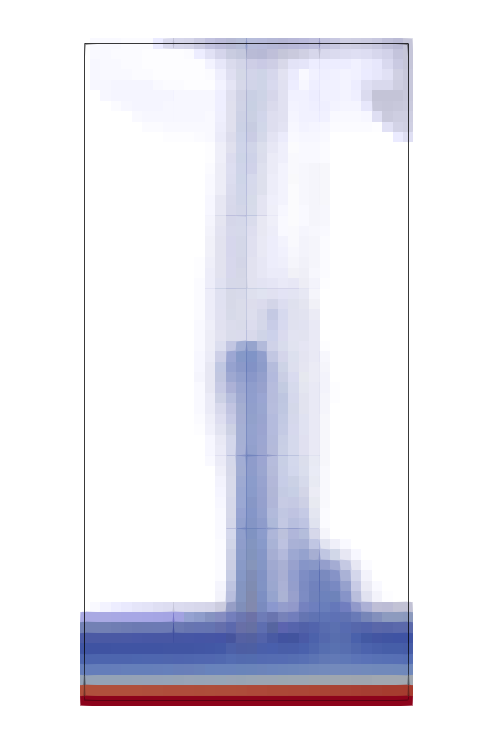
\includegraphics[width=80mm]{center_smoke.png}
\caption{ParaViewを用いて可視化した様子}
\label{fig:fig1}
%\end{center}
\end{figure}
\cite{fedkiew}を参考に格子法を用いた煙のシミュレーション手法を実装した.解像度は$32\times32\times64$に設定し,シミュレーション領域の1つの面に気体を配置し,配置した面の中心に熱源を置いて,煙が上昇する様子をシミュレーションした.図\ref{fig:fig1}は,圧力項計算に中心差分を用いた結果を,ParaViewを用いて可視化したものである.中心差分は誤差が二次精度であり精度面で優れるが,計算が安定しない問題がある.計算が安定しない風上差分に代わり,シミュレーションによく用いられる差分に風上差分がある.風上差分は誤差が一次精度であり,この誤差は粘性項と似ているため数値粘性と呼ばれる.粘性項の計算をこの数値粘性で代用することがある.
\section{今後の研究計画}
\cite{GPU}を参考に,離散コサイン変換を利用した展開圧縮手法を実装する.次にGPUの並列計算に対応させ,解像度$256\times512\times256$や,$1024\times1024\times1024$の高解像度のシミュレーションを実装する.実装を通じて煙の高解像度のシミュレーションの改善点を模索する.
% 参考文献
\begin{thebibliography}{99}

\bibitem{fedkiew}
R. FEDKIW, J. STAM, H. JENSEN. Visual simulation of smoke. In \textit{Proceedings of the 28th Annual Conference on Computer Graphics and Interactive Techniques}, SIGGRAPH ’01, pp. 15--22, 2001.

\bibitem{semi-Lagrangian}
J. STAM. Stable fluids. In \textit{Proceedings of the 26th Annual Conference on Computer Graphics and Interactive Techniques}, SIGGRAPH ’99, pp. 121--128 1999.

\bibitem{projection}
A. Chorin. A numerical method for solving incompressible viscous flow problems. \textit{Journal of Computational Physics}, 2:12--26, 1967.

\bibitem{GPU}
D. Ishida , R. Ando , S. Morishima. GPU smoke simulation on compressed DCT space. \textit{Eurographics - Short Papers}, 2019. DOI: 10.2312/egs.20191001.

\end{thebibliography}
\end{document}
